\section{Perceptrons \& MLP}

\begin{frame}{O Modelo de McCullogh e Pitts}

  \begin{figure}[t]
    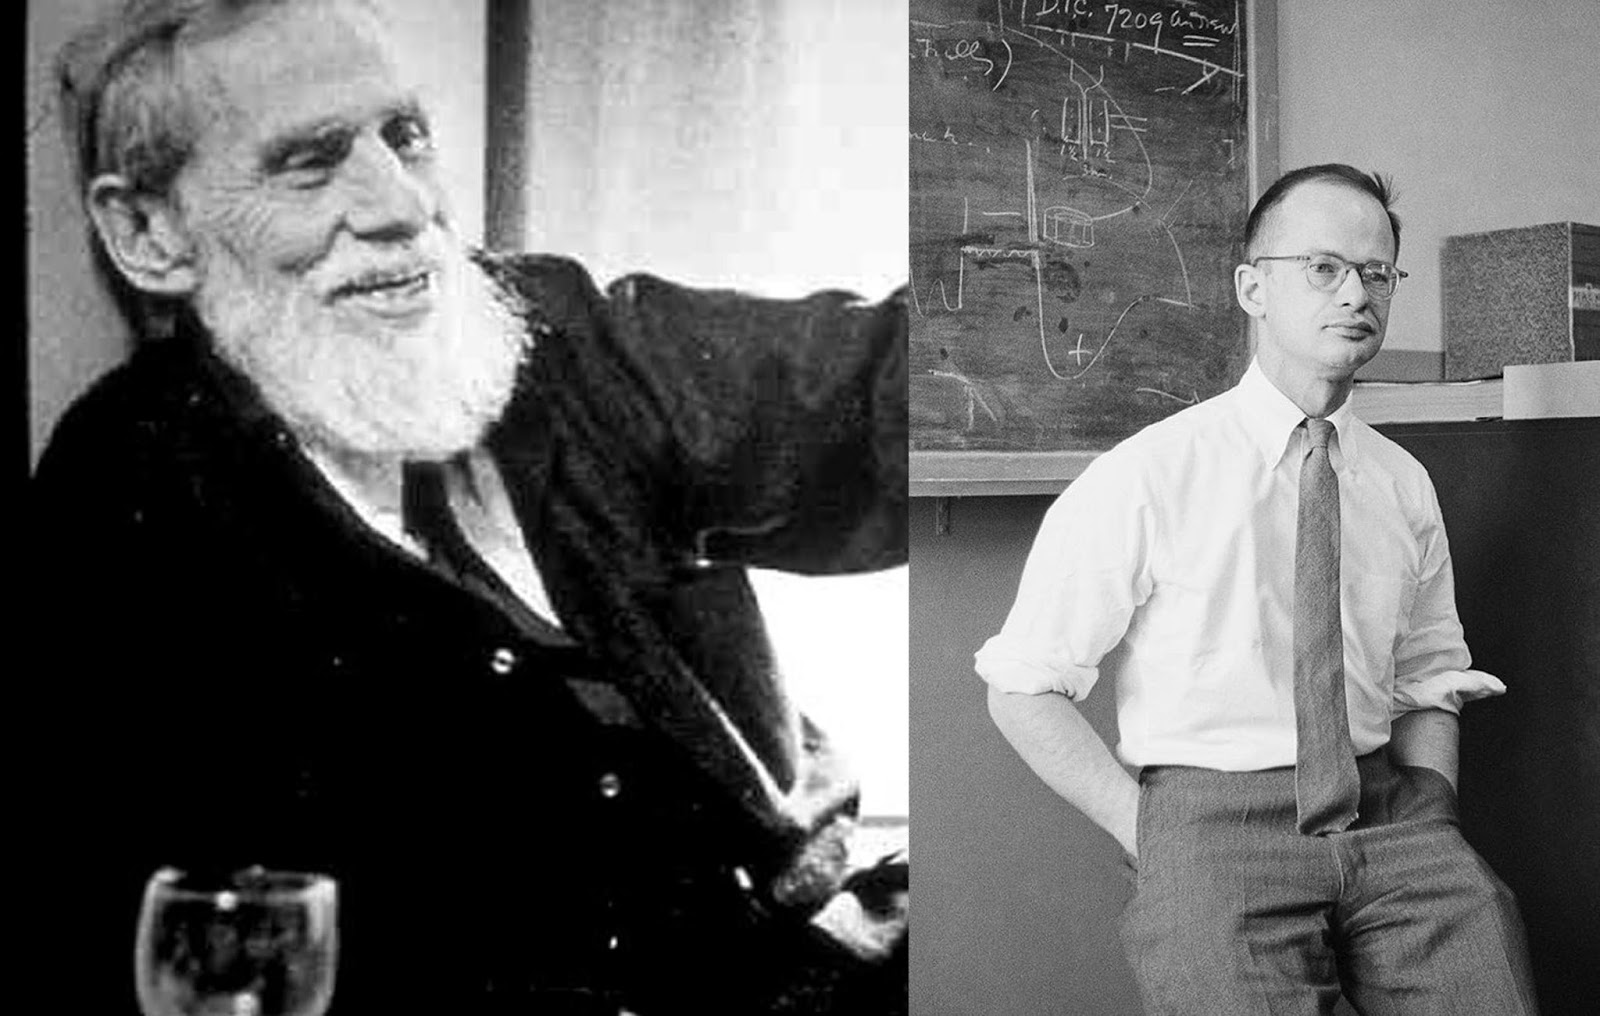
\includegraphics[width=0.8\textwidth]{warren_pitts.jpeg}
    \centering
  \end{figure}

\end{frame}

\begin{frame}{O Modelo de McCullogh e Pitts}

  \begin{figure}[t]
    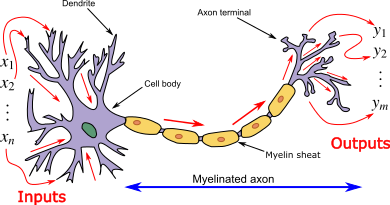
\includegraphics[width=0.8\textwidth]{neuron3.png}
    \caption{Neurônio biológico}
    \centering
  \end{figure}

\end{frame}

\begin{frame}{O Modelo de McCullogh e Pitts}

  \begin{figure}[t]
    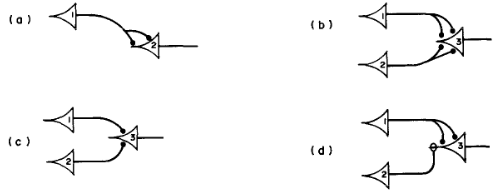
\includegraphics[width=\textwidth]{neuron1.png}
    \caption{Fonte: \cite{mcculloch1943logical}}
    \centering
  \end{figure}

\end{frame}

\begin{frame}{Aprendizado de Hebb}

  Quando um neurônio $x_i$ repetidamente ativa um neurônio $y$ a
  conexão entre $x_i$ e $y$ fica mais forte:

  \[ w_{i} = w_{i} + \eta x_i y \]

  \pause

  \begin{itemize}
    \item Conexões fortes apenas se reforçam (os pesos nunca se reduzem).
    \item Não existe noção de \"competição\" ou de limites pro aprendizado.
  \end{itemize}

\end{frame}

\begin{frame}{Aprendizado de Hebb (Generalizado)}

  \[ w_{ij} = w_{ij} + \eta y_j \left(x_i - \sum_{k=1}^{j} w_{ik}y_{k} \right)\]

  Um input é distribuido de forma incremental nos múltiplos outputs.

\end{frame}

\begin{frame}{Perceptron - Rosenblatt}

  \begin{figure}
    \begin{tikzpicture}
      \node[functions] (center) {};
      \node[below of=center,font=\scriptsize,text width=4em] (threshold) {Função de Ativação};
      \draw[thick] (0.5em,0.5em) -- (0,0.5em) -- (0,-0.5em) -- (-0.5em,-0.5em);
      \node[output, right=1.5em of center] (Y) {Y};
      \draw (0em,0.75em) -- (0em,-0.75em);
      \draw (0.75em,0em) -- (-0.75em,0em);
      \node[right of=center] (right) {};
        \path[draw,->] (center) -- (right);
      \node[functions,left=3em of center] (left) {$\sum$};
        \path[draw,->] (left) -- (center);
      \node[weights,left=3em of left] (2) {$w_2$} -- (2) node[input,left of=2] (l2) {$x_2$};
        \path[draw,->] (l2) -- (2);
        \path[draw,->] (2) -- (left);
      \node[below of=2] (dots) {$\vdots$} -- (dots) node[left of=dots] (ldots) {$\vdots$};
      \node[weights,below of=dots] (n) {$w_n$} -- (n) node[input,left of=n] (ln) {$x_n$};
        \path[draw,->] (ln) -- (n);
        \path[draw,->] (n) -- (left);
      \node[weights,above of=2] (1) {$w_1$} -- (1) node[input,left of=1] (l1) {$x_1$};
        \path[draw,->] (l1) -- (1);
        \path[draw,->] (1) -- (left);
      \node[weights,above of=1,fill=red!150!green!10] (0) {$w_0$} -- (0) node[input,left of=0,fill=red!150!green!10] (l0) {$x_0$};
        \path[draw,->] (l0) -- (0);
        \path[draw,->] (0) -- (left);
      \node[below of=ln,font=\scriptsize] {Inputs};
      \node[below of=n,font=\scriptsize] {Pesos};
    \end{tikzpicture}
  \centering
  \end{figure}

\begin{align}
Y = \left\{
  \begin{array}{cc}
    1 & \text{ se } \sum_{i=0}^{n} w_i x_i - T > 0 \\
    0 & \text{ caso contrário } \\
  \end{array} \right.
\end{align}

\end{frame}

\begin{frame}{Perceptron (1958) - Ajustando os pesos}

Seja $m$ o número de iterações.
\begin{align*}
  S(m) &= \sum_{i=0}^{n} w_i^m x_i^m \\
       &= \trans{\vt{w}}_m \vt{x}_m
\end{align*}

\begin{itemize}
  \item Se $\vt{x}_m$ é classificado de forma correta:
    \[ \vt{w}_{m+1} = \vt{w}_m \]
  \item Caso contrário, seja $\eta(m)$ uma taxa de aprendizado variando em $m$:
    \[ \vt{w}_{m+1} = \vt{w}_m - \eta(m) \vt{x}_m \]
\end{itemize}


\end{frame}

\begin{frame}{Perceptron (1958) - F.Rosenblatt}
  Consegue aprender:
  \begin{itemize}
    \item Funções booleanas.
    \item Atualiza os pesos quando encontra uma resposta errada.
    \item Rosenblatt provou formalmente que o algoritmo converge para problemas linearmente separáveis.
  \end{itemize}
\end{frame}

\begin{frame}{Perceptron - Rosenblatt}

  \begin{figure}
    \begin{tikzpicture}
    \node [input] (A) at (0,0)  {X};
    \node [input] (B) at (0,-2) {Y};
    \node [input] (C) at (3,-1) {1};
    \node [output, scale=0.5] (D) at (4.5,-1) {X $\lor$ Y};
    \path (A) edge node[above]{1} (C);
    \path (B) edge node[above]{1} (C);
    \path[draw, ->] (C) -- (D);
    \end{tikzpicture}
  \centering
  \end{figure}

  \begin{figure}
    \begin{tikzpicture}
    \node [input] (A) at (0,0)  {X};
    \node [input] (B) at (0,-2) {Y};
    \node [input] (C) at (3,-1) {2};
    \node [output, scale=0.5] (D) at (4.5,-1) {X $\land$ Y};
    \path (A) edge node[above]{1} (C);
    \path (B) edge node[above]{1} (C);
    \path[draw, ->] (C) -- (D);
    \end{tikzpicture}
  \centering
  \end{figure}

\end{frame}

\begin{frame}{Perceptron (1958) - F.Rosenblatt}
  \begin{block}{The New York Times (1958) \cite{olazaran1996sociological}}
    The Navy revealed the embryo of an electronic computer today that it expects will be able to walk, talk, see, write, reproduce itself and be conscious of its existence. Later perceptrons will be able to recognize people and call out their names and instantly translate speech in one language to speech and writing in another language, it was predicted.
  \end{block}
\end{frame}

\begin{frame}{Perceptrons (1969) - Minsky \& Papert}

  \begin{figure}
    \begin{tikzpicture}
    \node [input] (A) at (0,0)  {X};
    \node [input] (B) at (0,-2) {Y};
    \node [input] (C) at (3,-1) {?};
    \node [output, scale=0.5] (D) at (4.5,-1) {X $\oplus$ Y};
    \path (A) edge node[above]{?} (C);
    \path (B) edge node[above]{?} (C);
    \path[draw, ->] (C) -- (D);
    \end{tikzpicture}
  \centering
  \end{figure}

\end{frame}

\begin{frame}{Perceptrons (1969) - Minsky \& Papert}

  \begin{figure}
    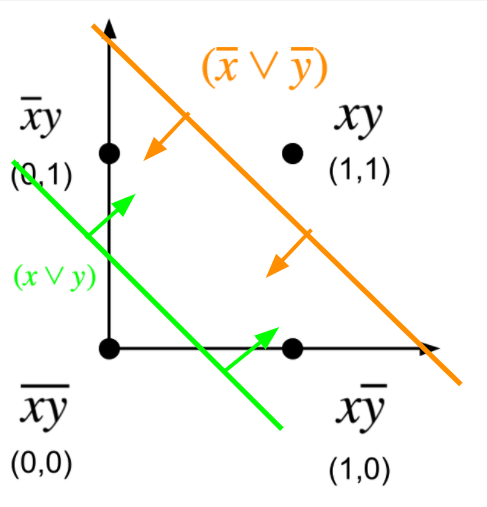
\includegraphics[width=0.55\linewidth]{minsky2.png}
  \end{figure}

  \begin{itemize}
    \item A Pesquisa sobre Perceptrons entrou em declínio em 1969, quando Marvin Minsky e Seymour Papert publicaram o livro "Perceptrons", onde eles descreveram algumas limitações do modelo.
  \end{itemize}

\end{frame}

\begin{frame}{Multi-Layer Perceptrons (1969) - Minsky \& Papert}

  \begin{figure}
    \begin{tikzpicture}
    \node [input] (A) at (0,0)  {X};
    \node [input] (B) at (0,-2) {Y};
    \node [input] (C) at (3,0)  {};
    \node [input] (D) at (3,-2) {};
    \node [output, scale=0.5] (E) at (5,-1) {X $\oplus$ Y};
    \path (A) edge node[above]{?} (C);
    \path (A) edge node[above]{?} (D);
    \path (B) edge node[below]{?} (C);
    \path (B) edge node[above]{?} (D);
    \path[draw, ->] (C) -- (E);
    \path[draw, ->] (D) -- (E);
    \end{tikzpicture}
  \centering
  \end{figure}

\end{frame}

\begin{frame}{The Universal Approximation Theorem}
  \begin{figure}[t]
    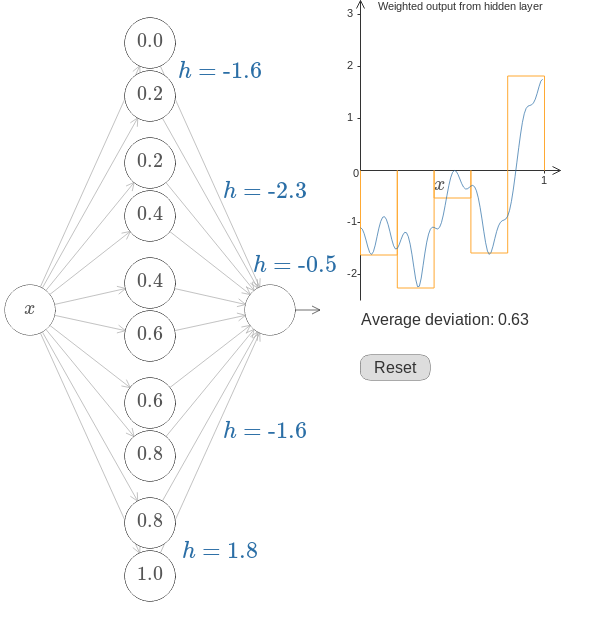
\includegraphics[width=0.7\textwidth]{uat00.png}
    \centering
  \end{figure}
\end{frame}
